
\chapter{NB-IOT通信模块设计}
\section{模块总体介绍}

上海移远通信技术有限公司开发的bc35G通信模组支持 band8、band5、band20、band28频段,采用LCC贴片封装,尺寸为19.9mm*23.6mm*2.2mm,完全符合欧盟RoHs标准(TODO:引用),外部参数如下:
模块参数

\begin{figure}[h]
	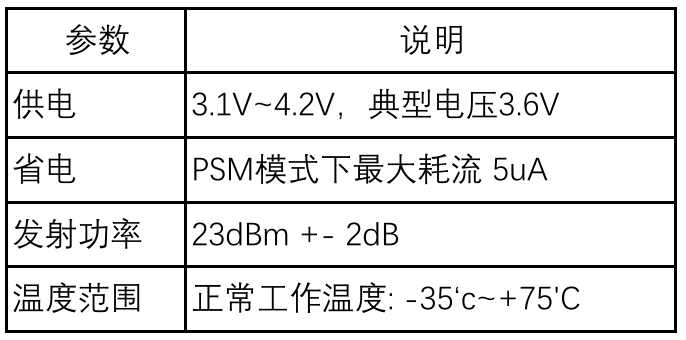
\includegraphics[width=8cm]{模块参数.png}
	\caption{模块参数}
	\label{模块参数}
\end{figure}

模块总体

\begin{figure}[h]
    \floatcontinue
	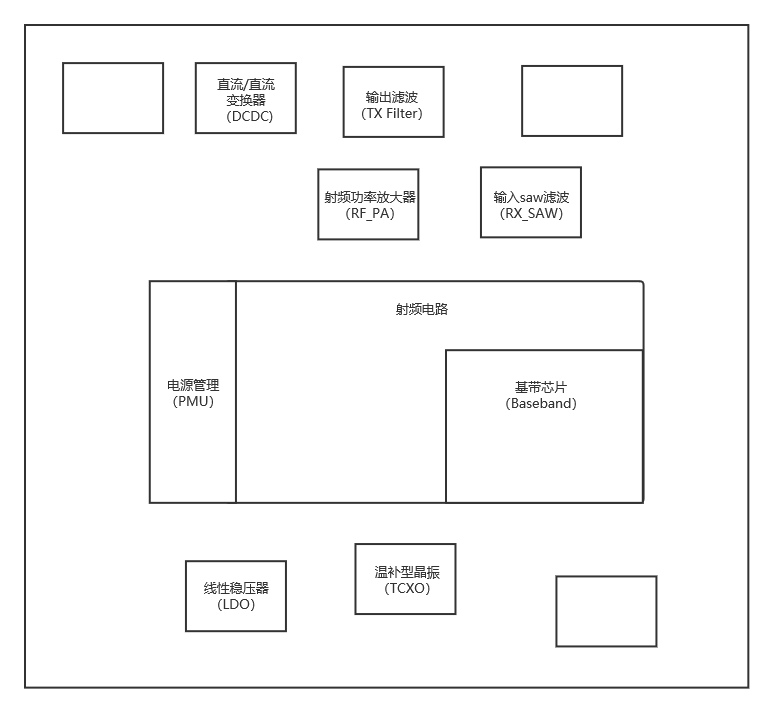
\includegraphics[width=13cm]{总体框图.png}
	\caption{总体框图}
	\label{总体框图}
\end{figure}


\section{供电}
为了将锂离子电池电压转化为模块供电电压3.1v~4.2v,选用低压降线性稳压器(LDO),具有成本低,噪音低的优点。同时由于对电池能量损耗低,保证更长的工作时间。在靠近模块的VBAT输入端,并联一个100uF的钽电容,以及100nF、100pF和22pF的滤波电容。同时为了提高模块承受浪涌电压的能力,在VBAT输入端增加一个TVS管。
输入端参考电路如下:(TODO:图片)

\section{串口}
bc35g模块提供两对串口,分别为主串口和调试串口。主串口用于AT命令的通信、数据传输,在Active、Idle和PSM模式下均可工作。模块作为DCE,连接方式为:(TODO:图片:DCT-DTE连接)
通过RS323电平转化芯片与MCU连接,为了降低串口功耗,在模块和主机之间加上1k欧姆电阻用于降低串口电流(TODO:RS232连接图)

\section{射频模块}
BC35G天线部分预留了pi型匹配电路(TODO:图片),以便对天线性能调节。C1和C2两个电容将大多数交流成分滤除,R1为0欧电阻,充当pi型RC滤波电路的电感。为了确保射频信号的性能以及可靠性,需要遵循pi型匹配电路的layout。既要保证电容电感布局靠近,也要防止出现stub(TODO:引用)

\section{USIM卡座}
支持3GPP规范功能的USIM卡能接入运营商网络,USIM功能包括模块和卡座,为了确保USIM卡的性能以及避免与射频、电源模块的干扰,须遵循以下设计原则:
卡座和模块尽量靠近,信号线不超过200mm保证信号品质
信号线远离RF走线及VBAT
防止USIM\_DATA和USIM\_CLK信号干扰,两线之间加入地屏蔽
USIM\_DATA, USIM\_VDD, USIM\_CLK, 和USIM\_RST并联33pF电容滤除RF干扰
为了防止静电,在卡座和模块之间增加TVS管

USIM卡使用内部电源3v供电,引脚定义如下:(TODO:表格)

USIM卡座电路图:(TODO:图片)

\subsection{时域积分方程时间步进算法产生的阻抗矩阵的特征}
由于时域混合场积分方程是时域电场积分方程与时域磁场积分方程的线性组合,因此时域混合场积分方程时间步进算法的阻抗矩阵特征与时域电场积分方程时间步进算法的阻抗矩阵特征相同。

\subsection{数值算例与分析}

如图3-1(a)所示给出了时间步长选取为0.5ns时采用三种不同存储方式计算的平板中心处 方向的感应电流值与IDFT方法计算结果的比较。如图3-1(b)所示给出了存储方式为基权函数压缩存储方式,时间步长分别取时平板中心处 方向的感应电流计算结果,从图中可以看出不同时间步长的计算结果基本相同。

\begin{algorithm}[H]
 \KwData{this text}
 \KwResult{how to write algorithm with \LaTeX2e }
 initialization\;
 \While{not at end of this document}{
  read current\;
  \eIf{understand}{
   go to next section\;
   current section becomes this one\;
   }{
   go back to the beginning of current section\;
  }
 }
 \caption{How to wirte an algorithm.}
\end{algorithm}

由于时域混合场积分方程是时域电场积分方程与时域磁场积分方程的线性组合,因此时域混合场积分方程时间步进算法的阻抗矩阵特征与时域电场积分方程时间步进算法的阻抗矩阵特征相同。

\section{时域积分方程时间步进算法矩阵方程的求解}

\section{本章小结}
本章首先研究了时域积分方程时间步进算法的阻抗元素精确计算技术,分别采用DUFFY变换法与卷积积分精度计算法计算时域阻抗元素,通过算例验证了计算方法的高精度。